\documentclass{article} % PDFTex, XeLaTex 都支持。

% 中文环境
%\documentclass[hyperref, UTF8]{ctexart} %若选择{ctexart}则直接支持中文,下面的{ctex}要去掉。
%\usepackage[UTF8]{ctex} %中文配置。
%\usepackage[UTF8, heading=false, scheme=plain]{ctex} %加入scheme=plain,行距、中西文公共字符都有变化。

% 版面设置
\usepackage{geometry}
\geometry{a4paper}

% 额外的功能
\usepackage{authblk} %添加机构,需要安装preprint包
\usepackage{amsthm} %证明环境
\usepackage{amsmath} %数学公式
\numberwithin{equation}{section} % 公式按章节编号
\usepackage{amssymb}
\usepackage{multirow} % multirow
\usepackage{booktabs} % toprule, midrule, bottomrule

% 表格的单元格内换行、对齐功能
\usepackage{makecell}

% 图片支持
\usepackage{graphicx} %添加图片
\graphicspath{{figures/}}
\usepackage{float} % 控制图片是否浮动:[htbp]浮动,或[H]禁止浮动

% PDF索引及超链接 (black,red,blue,green)
\usepackage[colorlinks=true,linkcolor=black,anchorcolor=black,citecolor=blue,filecolor=black,menucolor=black,runcolor=black,urlcolor=black]{hyperref}

% 首行缩进
\usepackage{indentfirst} % 首行缩进支持
\setlength{\parindent}{2em} % 首行缩进两个汉字

% 列表样式定制
\usepackage{enumerate}
\usepackage{enumitem}
\setlist[enumerate,1]{label=(\arabic*).,font=\textup,leftmargin=14mm,labelsep=1.5mm,topsep=0mm,itemsep=-0.8mm}
\setlist[enumerate,2]{label=(\alph*).,font=\textup,leftmargin=14mm,labelsep=1.5mm,topsep=-0.8mm,itemsep=-0.8mm}
%\setlist{nosep} % 取消行间空行

% 自定义命令
\newcommand{\SL}{\rule{.3em}{.3pt}} % 定义短下划线

% 名称、作者、机构
\title{Formal Method Library for Propulsion System of FCS}
\author{Zhengpu Shi}
\affil{Draft V1.0}
%\affil{南京航空航天大学}
\date{Oct 25, 2020} %注释后显示为编译时日期


\begin{document}

% 生成标题
\maketitle
\newpage
% ++++++++++++++++++++++++++++++++++++++++++++++++++++++++++++++++++++++++++++++++++++++++++++++++++

% 生成目录
\tableofcontents
\newpage
% ++++++++++++++++++++++++++++++++++++++++++++++++++++++++++++++++++++++++++++++++++++++++++++++++++

%\listoffigures
%\newpage
% 生成图片列表,请删除上面两行注释

%\begin{figure}[H]%[htbp]
%\centering\includegraphics[scale=0.85]{graph.jpg}
%\centerline{\includegraphics[width=1.0\textwidth]{graph.jpg}}
%\caption{this is a figure demo}
%\label{fig:label}
%\end{figure}

\section{Introduction}
This is one part of the FML4FCS project. 
For detail information, please refer the introduction of the whole project in this website.


\newpage
% ++++++++++++++++++++++++++++++++++++++++++++++++++++++++++++++++++++++++++++++++++++++++++++++++++

\section{Propulsion System (PS)}

The modeling of Propulsion System (we called PS) is a basic condition for designing the flight control system.

We set up a module named Common Module which related to the general issues.
Then we set up some modules named like Example* Module for several specific problems.

\subsection{Common Module}

\subsubsection{Definition of constants}
Constants refer to values that do not change after the aircraft is designed, such as propeller size.
We have slightly simplified the aerodynamics, and set the flight altitude and ambient temperature to constants, so the air pressure and air density also become constants. 
The reason for this is that their changes during low-altitude flight are very small, almost negligible, and in order to highlight other more important variables, simplifying them to constants will make the entire model more concise.

Although the Coq system supports to using Unicode characters as identifier, we still use ASCII text represent an identify.
Because other languages may not support this feature and we need to maintain naming consistency.


{\footnotesize
\begin{tabular}{c|c|r|c|l}
\toprule
\textbf{Symbol} 		& \textbf{Identifier} & \textbf{Meaning} 			& \textbf{Unit} 	& \textbf{Remark} \\
\midrule
\multicolumn{5}{c}{E N V I R O N M E N T}\\ 
\hline
$T_0$ 					& T\_0 			& standard temperature				& $K$   			& 273.15K	\\
$p_0$					& p\_0 			& standard atmospheric pressur		& $Pa$				& $101.325\times10^5$	\\ 
$\rho_0$				& rho\_0 		& standard atmospheric density		& $kg/m^3$			& 1.293	\\
$h$						& h 			& Altitude							& $m$				& \\
$T_t$					& T\_t 			& Environment temperature			& $^{\circ}$C		& \\
$n_r$					& n\_r 			& Number of rotors					& $piece$			& \\
$G$						& G 			& Total weight	 					& $N$ 				& \\
$I_{other}$				& I\_other		& Other current	 					& $A$ 				& \\
$p$						& p 			& atmospheric pressure				& $Pa$				& \\
$\rho$					& rho 			& density							& $kg/m^3$			& \\
\hline
\multicolumn{5}{c}{P R O P E L L E R}\\ 
\hline
$D_p$					& D\_p 			& Propeller diameter				& $m$				& \\
$H_p$					& H\_p 			& Propeller geometric pitch			& $m$				& \\
$B_p$					& B\_p 			& Number of blades					& $piece$			& \\
$G_p$      		       	& G\_p			& Propeller weight                  & $N$          		& \\
$PP_A$     		   		& PP\_A			& Propeller parameter*        		& -          		& \cite{qq}[p67]\\
$PP_\varepsilon$ 	   	& PP\_epsilon	& Propeller parameter*        		& -          		& \cite{qq}[p67]\\
$PP_\lambda$     	   	& PP\_lambda	& Propeller parameter*        		& -          		& \cite{qq}[p67]\\
$PP_\zeta$       	   	& PP\_zeta		& Propeller parameter*        		& -          		& \cite{qq}[p67]\\
$PP_e$           	   	& PP\_e			& Propeller parameter*        		& -          		& \cite{qq}[p67]\\
$PP_{K0}$        	   	& PP\_K0		& Propeller parameter*        		& -          		& \cite{qq}[p67]\\
$PP_{\alpha0}$   	   	& PP\_alpha0	& Propeller parameter*        		& -          		& \cite{qq}[p67]\\
$C_{fd}$         	    & C\_fd			& Zero-lift drag coefficient    	& -          		& \\
$C_T$					& C\_T 			& Thrust coefficient				& $-$				& \\
$C_M$					& C\_M 			& Torque coefficient				& $-$				& \\
$C_d$					& C\_d 			& Drag coefficient					& $-$				& \\
\hline
\multicolumn{5}{c}{M O T O R}\\ 
\hline
$K_{V0}$				& K\_V0 		& Nominal no-load motor KV			& $r/min/V$			& \\
$U_{m0}$				& U\_m0 		& Nominal no-load motor voltage		& $V$				& \\
$I_{m0}$				& I\_m0 		& Nominal no-load motor current		& $A$				& \\
$I_{mMax}$				& I\_mMax		& Maximum motor input current		& $A$				& \\
$R_m$					& R\_m 			& Motor resistance					& $\Omega$			& \\
$G_{m}$          		& G\_m 			& Motor weight                      & $N$          		& \\
$K_E$					& K\_E 			& Back-electromotive force constant & $-$				& \\
$K_T$					& K\_T 			& Torque constant					& $-$				& \\
\hline
\multicolumn{5}{c}{E S C}\\ 
\hline
$I_{eMax}$				& I\_eMax		& Maximum ESC output current		& $A$				& \\
$R_{e}$					& R\_e 			& ESC resistance					& $\Omega$			& \\
$G_e$            		& G\_e 			& ESC weight                        & $N$          		& \\
\hline
\multicolumn{5}{c}{B A T T E R Y}\\ 
\hline
$R_{b}$					& R\_b 			& Battery resistance				& $\Omega$			& \\
$U_{b}$					& U\_b 			& Battery voltage					& $V$				& \\
$C_{b}$					& C\_b 			& Battery capacity					& $mAh$				& \\
$C_{min}$				& C\_min 		& Battery minimum capacity			& $mAh$				& \\
$K_{b}$					& K\_b 			& Maximum discharge rate			& $C$				& \\
$G_b$            		& G\_b 			& Battery weight                    & $N$          		& \\
\bottomrule
\end{tabular}
\label{tab:basic_constant}
}

Notice that, some constants are composed by more basic constants. We give all the relationship of them.

Definition of $p$, see \cite{qq}[p.66, 4.4]
\begin{equation}
p=p_0 \left( 1-0.0065 \frac {h}{T_0+T_t } \right)  ^{5.2561} \label{basic.p}
\end{equation}

Definition of $\rho$, see \cite{qq}[p.66, 4.3]
\begin{equation}
\rho=\frac {T_0 p}{p_0 (T_0+T_t) } \rho_0 \label{basic.rho_0}
\end{equation}

Definition of $C_T$, see \cite{qq}[p.67, 4.6]
\begin{equation}
C_T = 0.25\pi^3\lambda\zeta^2 B_p K_0 \frac{\varepsilon arctan \frac{H_p}{\pi D_P} - \alpha_0}{\pi A + K_0} \label{basic.C_T}
\end{equation}

Definition of $C_d$, see \cite{qq}[p.67, 4.7]
\begin{equation}
C_d = C_{fd} + \frac {\pi A K_0^2} {e} 
\frac {\left(\varepsilon\arctan{\frac {H_p}{\pi D_p}}-\alpha_0\right)^2} {\left(\pi A + K_0\right)^2} \label{basic.C_d}
\end{equation}

Definition of $C_M$, see \cite{qq}[p.67, 4.6]
\begin{equation}
C_M = \frac{1}{8A}\pi^2 C_d\zeta^2 \lambda B_p^2 \label{basic.C_M}
\end{equation}

Definition of $K_E$, see \cite{qq}[p.80, 4.64]
\begin{equation}
K_{E} = \frac {U_{m0} - I_{m0} R_m} {K_{V0} U_{m0}} \label{basic.K_E}
\end{equation}

Definition of $K_T$, see \cite{qq}[p.80, 4.65]
\begin{equation}
K_{T} = 9.55 K_{E} \label{basic.K_T}
\end{equation}


\subsubsection{Definition of variables}

Variable means that its value may changed at different or in different problems. 

{\footnotesize
\begin{tabular}{c|c|r|c|l}
\toprule
\textbf{Symbol} 		& \textbf{Identifier} & \textbf{Meaning} 			& \textbf{Unit} 	& \textbf{Remark} \\
\hline
\multicolumn{5}{c}{E N V I R O N M E N T}\\ 
\hline
$p$       		  		& p				& atmospheric pressure              & $Pa$         		& \\
$\rho$    		  		& rho			& density                           & $kg/m^3$   		& \\
$T_b$      				& T\_b			& Time of endurance                 & $min$        		& \\
$V$        				& V				& Flight speed                      & $m/s$        		& \\
$V_{max}$  				& V\_max		& Maximum flight speed              & $m/s$        		& \\
$Z$        				& Z				& Flight distance                   & $m$          		& \\
$Z_{max}$  				& Z\_max		& Maximum flight distance           & $m$          		& \\
$\eta$  				& eta			& System efficiency           		& $m$          		& 0\~{}1 \\
$G_{maxload}$			& G\_maxload	& Maximum load		           		& $N$          		& \\
$\theta_{max}$			& theta\_max	& Maximum pitch angle          		& $rad$        		& \\
\hline
\multicolumn{5}{c}{P R O P E L L E R}\\ 
\hline
$T$              		& T				& Propeller thrust                  & $N$          		& \\
$M$              		& M				& Propeller torque                  & $N.m$        		& \\
$N$              		& N				& Motor speed                       & $r/min$      		& \\
\hline
\multicolumn{5}{c}{M O T O R}\\ 
\hline
$E_a$            		& E\_a			& Back-electromotive force          & $V$        	  	& \\
$U_m$            		& U\_m			& Equivalent motor input voltage    & $V$        	  	& \\
$I_m$            		& I\_m			& Equivalent motor input current    & $A$        	  	& \\
\hline
\multicolumn{5}{c}{E S C}\\ 
\hline
$I_e$            		& I\_e			& ESC input current                 & $A$    	      	& \\
$U_e$            		& U\_e			& ESC input voltage                 & $V$     	     	& \\
$U_{eo}$         		& U\_eo			& Equivalent ESC output voltage     & $V$      	    	& \\
$\sigma_e$       		& sigma\_e		& ESC throttle                      & -        		  	& 0\~{}1 \\
\hline
\multicolumn{5}{c}{B A T T E R Y}\\ 
\hline
$I_b$            		& I\_b			& Battery current                   & $A$          		& \\
\bottomrule
\end{tabular}
}

\subsubsection{Variable Relation Graph (VRG) }

We study the engineering relationship between the various components of the PS, and give the VRG of the most important 14 variables in Fig \ref{fig:fig1_VariableFlow}, which can help us visually design function expressions between the variables.

Here is the dependency relationship between all variables. 
From this picture, you can intuitively see how to calculate between two variables or multiple variables.
The double-headed arrow means that two variables can be freely converted.
The dashed line represents the derived simple relationship.
A one-way arrow refers to a situation where there are multiple inputs and a single output. 
Although the reverse solution cannot be obtained directly, because there are also relationships between the input variables, the solution process can still be constructed.

This picture can help us deal with the forward and reverse problems in the propulsion system.
Forward solution refers to solving the aircraft's performance indicators (longest hovering time, maximum load, maximum pitch angle, etc.) based on known hardware parameters (propeller, motor, ESC, battery, etc.).
The reverse solution is to solve the hardware parameters according to the given aircraft performance index.

\begin{figure}[H]%[htbp]
\centerline{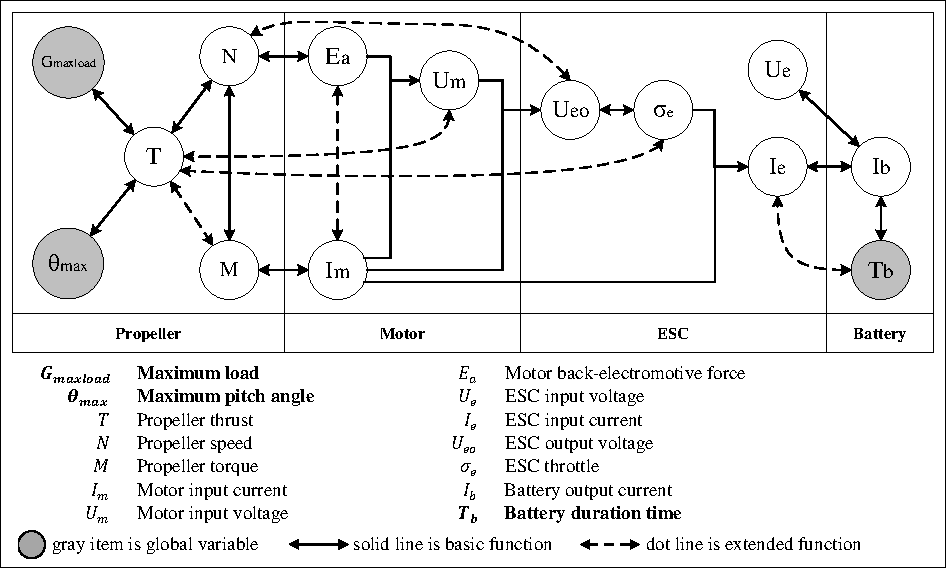
\includegraphics[width=1.0\textwidth]{fig1_VariableFlow.pdf}}
\caption{Variable Relationship Graph of Propulsion Subsystem}
\label{fig:fig1_VariableFlow}
\end{figure}

The graph is divided into four parts, namely the propeller, motor, ESC and battery.
Each circle in the graph represents a variable, and the connection represents a function.
It can be seen from the graph that there is a one-to-one function obtained by one or more steps between any nodes, although some function forms can be more complex.

\subsubsection{Definition of basic functions}\label{main:basic:basic_functions}

Basic functions are given by engineering principles that describe the most basic conversion relationship between variables. 

Calculate $T$ by $N$, see \cite{qq}[p.66, 4.1]
\begin{equation}
get\SL T\SL by\SL N (N) = \rho C_T D_P^4 \left(\frac N {60} \right)^2 \label{basic.get_T_by_N}
\end{equation}

Calculate $M$ by $N$, see\cite{qq}[p.66, 4.2]
\begin{equation}
get\SL M\SL by\SL N (N) = C_M\rho \left(\frac N {60} \right)^2 D_P^5 \label{basic.get_M_by_N}
\end{equation}

Calculate $E_a$ by $N$, see\cite{qq}[p.80, 4.61]
\begin{equation}
get\SL E\SL a\SL by\SL N (N) = K_{E} N \label{basic.get_E_a_by_N}
\end{equation}

Calculate $M$ by $I_m$, see\cite{qq}[p.80, 4.59]
\begin{equation}
get\SL M\SL by\SL I\SL m (I_m) = K_T (I_m - I_{m0}) \label{basic.get_M_by_I_m}
\end{equation}

Calculate $U_m$ by $E_a$ and $I_m$, see\cite{qq}[p.72]
\begin{equation}
get\SL U\SL m\SL by\SL E\SL a\SL and\SL I\SL m (E_a, I_m) = E_a + R_m I_m \label{basic.get_U_m_by_E_a_and_I_m}
\end{equation}

Calculate $U_{eo}$ by $U_m$ and $I_m$, see\cite{qq}[p.69, 4.12]
\begin{equation}
get\SL U\SL eo\SL by\SL U\SL m\SL and\SL I\SL m (U_m, I_m) = U_m + I_m R_e\label{basic.get_U_eo_by_U_m_and_I_m}
\end{equation}

Calculate $U_{eo}$ by $sigma_e$, see\cite{qq}[p.69, 4.13]
\begin{equation}
get\SL U\SL eo\SL by\SL sigma\SL e (sigma_e) = sigma_e U_b \label{basic.get_U_eo_by_sigma_e}
\end{equation}

Calculate $I_e$ by $sigma_e$ and $I_m$, see\cite{qq}[p.69, 4.14]
\begin{equation}
get\SL I\SL e\SL by\SL sigma\SL e\SL and\SL I\SL m (sigma_e, I_m) = \sigma_e I_m \label{basic.get_I_e_by_sigma_e_and_I_m}
\end{equation}

Calculate $I_b$ by $I_e$, see\cite{qq}[p.70, 4.17]
\begin{equation}
get\SL I\SL b\SL by\SL I\SL e (I_e) = n_r I_e + I_{other} \label{basic.get_I_b_by_I_e}
\end{equation}

Calculate $U_e$ by $I_b$, see\cite{qq}[p.70, 4.20]
\begin{equation}
get\SL U\SL e\SL by\SL I\SL b (I_b) = U_b - I_b R_b \label{basic.get_U_e_by_I_b}
\end{equation}

Calculate $T_b$ by $I_b$, see\cite{qq}[p.70, 4.22]. 
Notice that, we simplify the battery model. 
First, we assume the battery voltage is a fixed value when it is discharging.
Second, we assume the remain capacity of battery is linear changed when it is discharging.
\begin{equation}
get\SL T\SL b\SL by\SL I\SL b (I_b) = \frac{C_b-C_{min}}{I_b} \frac{60}{1000} \label{basic.get_T_b_by_I_b}
\end{equation}

Calculate $G_{maxload}$ by $T$, see\cite{qq}[p.74, 4.35]
\begin{equation}
get\SL G\SL maxload\SL by\SL T (T) = n_r T - G \label{basic.get_G_maxload_by_T}
\end{equation}

Calculate $\theta_{max}$ by $T$, see\cite{qq}[p.74, 4.36]
\begin{equation}
get\SL theta\SL max\SL by\SL T (T) = \arccos{\frac{G}{n_r T}} \label{basic.get_theta_max_by_T}
\end{equation}

Calculate $\eta$ by $M$ and $N$ and $I_b$, see\cite{qq}[p.73, 4.32]
\begin{equation}
get\SL eta\SL by\SL M\SL and\SL N\SL and\SL I\SL b (M, N, I_b) = \frac{\frac{2\pi}{60} n_r M N}{U_b I_b} \label{basic.get_eta_by_M_and_N_and_I_b}
\end{equation}


\subsubsection{Definitions of basic inverse functions}\label{main:basic:inverse_functions}
The basic inverse functions are some inverse functions of unary functions which belongs to basic function.

Calculate $N$ by $T$, it is an inverse function of \eqref{basic.get_T_by_N}.
\begin{equation}
get\SL N\SL by\SL T (T) = 60 \sqrt{\frac{T}{\rho C_T D_p^4}} \label{basic.get_N_by_T}
\end{equation}

Calculate $N$ by $M$, it is an inverse function of \eqref{basic.get_M_by_N}.
\begin{equation}
get\SL N\SL by\SL M (M) = 60 \sqrt{\frac{M}{\rho D_p^5 C_M}} \label{basic.get_N_by_M}
\end{equation}

Calculate $N$ by $E_a$, it is an inverse function of \eqref{basic.get_E_a_by_N}.
\begin{equation}
get\SL N\SL by\SL E\SL a (E_a) = \frac{E_a}{K_E} \label{basic.get_N_by_E_a}
\end{equation}

Calculate $I_m$ by $M$, it is an inverse function of \eqref{basic.get_M_by_I_m}.
\begin{equation}
get\SL I\SL m\SL by\SL M (M) = \frac{M}{K_T}+{I_{m0}} \label{basic.get_I_m_by_M}
\end{equation}

Calculate $sigma_e$ by $U_{eo}$, it is an inverse function of \eqref{basic.get_U_eo_by_sigma_e}.
\begin{equation}
get\SL sigma\SL e\SL by\SL U\SL eo (U) = \frac{U_{eo}}{U_b} \label{basic.get_sigma_e_by_U_eo}
\end{equation}

Calculate $I_e$ by $I_b$, it is an inverse function of \eqref{basic.get_I_b_by_I_e}.
\begin{equation}
get\SL I\SL e\SL by\SL I\SL b (I_e) = \frac{I_b - I_{other}}{n_r} \label{basic.get_I_e_by_I_b}
\end{equation}

Calculate $I_b$ by $U_e$, it is an inverse function of \eqref{basic.get_U_e_by_I_b}.
\begin{equation}
get\SL I\SL b\SL by\SL U\SL e (U_e) = \frac{U_b - U_e}{R_b} \label{basic.get_I_b_by_U_e}
\end{equation}

Calculate $I_b$ by $T_b$, it is an inverse function of \eqref{basic.get_T_b_by_I_b}.
\begin{equation}
get\SL I\SL b\SL by\SL T\SL b (T_b) = \frac{C_b - C_{min}}{T_b} \frac{60}{1000} \label{basic.get_I_b_by_T_b}
\end{equation}

Calculate $T$ by $G_{maxload}$, it is an inverse function of \eqref{basic.get_G_maxload_by_T}.
\begin{equation}
get\SL T\SL by\SL G\SL maxload (G_{maxload}) = \frac{G_{maxload} + G}{n_r} \label{basic.get_T_by_G_maxload}
\end{equation}

Calculate $T$ by $\theta_{max}$, it is an inverse function of \eqref{basic.get_theta_max_by_T}.
\begin{equation}
get\SL T\SL by\SL theta\SL max (\theta_{max}) = \frac{G}{n_r \cos{\theta_{max}}} \label{basic.get_T_by_theta_max}
\end{equation}


\subsubsection{Definitions of extended functions}\label{main:basic:extended_functions}
Extended function are some composited functions by basic functions and basic inverse functions, and the compositions are one or more steps.

Calculate $T$ by $M$, it is composed by \eqref{basic.get_N_by_M} and \eqref{basic.get_T_by_N}.
\begin{equation}
get\SL T\SL by\SL M (M) = \frac{C_T * M}{D_p C_M} \label{basic.get_T_by_M}
\end{equation}

Calculate $M$ by $T$, it is an inversion function of \eqref{basic.get_T_by_M}.
\begin{equation}
get\SL M\SL by\SL T (T) = \frac{C_M D_p T}{C_T} \label{basic.get_M_by_T}
\end{equation}

Calculate $I_m$ by $T$, it is composed by \eqref{basic.get_M_by_T} and \eqref{basic.get_I_m_by_M}.
\begin{equation}
get\SL I\SL m\SL by\SL T (T) = \frac{C_M D_p T}{K_T C_T} + I_{m0}  \label{basic.get_I_m_by_T}
\end{equation}

Calculate $T$ by $M$, it is composed by \eqref{basic.get_N_by_T} and \eqref{basic.get_E_a_by_N}.
\begin{equation}
get\SL E\SL a\SL by\SL T (T) = {60} K_E \sqrt{\frac{T}{\rho C_T D_p^4}}  \label{basic.get_E_a_by_T}
\end{equation}

Calculate $U_m$ by $T$, it is composed by \eqref{basic.get_E_a_by_T} and \eqref{basic.get_I_m_by_T} and \eqref{basic.get_U_m_by_E_a_and_I_m}.
\begin{equation}
get\SL U\SL m\SL by\SL T (T) = {60} K_E \sqrt{\frac{T}{\rho C_T D_p^4}} 
	+ R_m \left(\frac{C_M D_p T}{K_T C_T} + I_{m0}\right) \label{basic.get_U_m_by_T}
\end{equation}

Calculate $U_m$ by $N$ and $M$, it is composed by \eqref{basic.get_E_a_by_N} and \eqref{basic.get_I_m_by_M} and \eqref{basic.get_U_m_by_E_a_and_I_m}.
\begin{equation}
get\SL U\SL m\SL by\SL N\SL and\SL M (N, M) = K_E N 
	+ R_m \left(\frac{M}{K_T} + I_{m0}\right) 
	\label{basic.get_U_m_by_N_and_M}
\end{equation}

Calculate $U_m$ by $N$, it is composed by \eqref{basic.get_M_by_N} and \eqref{basic.get_U_m_by_N_and_M}.
\begin{equation} \label{basic.get_U_m_by_N}
get\SL U\SL m\SL by\SL N (N) = K_E N + R_m \left(\frac{ C_M\rho \left(\frac N {60} \right)^2 D_P^5 }{K_T} + I_{m0}\right)
\end{equation}

Calculate $U_m$ by $M$, it is composed by \eqref{basic.get_N_by_M} and \eqref{basic.get_U_m_by_N_and_M}.
\begin{equation}
get\SL U\SL m\SL by\SL M (M) = 60  K_E \sqrt{\frac{M}{\rho D_p^5 C_M}} 
	+ R_m \left(\frac{M}{K_T} + I_{m0}\right) 
	\label{basic.get_U_m_by_M}
\end{equation}

Calculate $I_m$ by $E_a$, it is composed by \eqref{basic.get_U_m_by_E_a_and_I_m} and \eqref{basic.get_U_eo_by_U_m_and_I_m}.
\begin{equation}
get\SL U\SL eo\SL by\SL E\SL a\SL and\SL I\SL m (E_a, I_m) = E_a + (R_m + R_e) I_m \label{basic.get_U_eo_by_E_a_and_I_m}
\end{equation}

Calculate $U_{eo}$ by $N$, it is composed by \eqref{basic.get_U_eo_by_U_m_and_I_m}, 
   \eqref{basic.get_U_m_by_E_a_and_I_m}, 
   \eqref{basic.get_E_a_by_N}, 
   \eqref{basic.get_I_m_by_M} and
   \eqref{basic.get_M_by_N}.
\begin{equation}
get\SL U\SL eo\SL by\SL N (N) = \frac{(R_m + R_e) C_M \rho D_p^5}{K_T 60^{2}} N^2
	+ K_E N + (R_m + R_e) I_{m0}
\end{equation}

Calculate $sigma_e$ by $E_a$ and $I_m$, it is composed by \eqref{basic.get_sigma_e_by_U_eo} and \eqref{basic.get_U_eo_by_E_a_and_I_m}.
\begin{equation}
get\SL sigma\SL e\SL by\SL E\SL a\SL and\SL I\SL m (E_a, I_m) = \frac{E_a + (R_m + R_e) I_m}{U_b} \label{basic.get_sigma_e_by_E_a_and_I_m}
\end{equation}

Calculate $I_e$ by $E_a$ and $I_m$, it is composed by \eqref{basic.get_sigma_e_by_E_a_and_I_m} and \eqref{basic.get_I_e_by_sigma_e_and_I_m}.
\begin{equation}
get\SL I\SL e\SL by\SL E\SL a\SL and\SL I\SL m (E_a, I_m) = \frac{(E_a + (R_m + R_e) I_m) I_m}{U_b} \label{basic.get_I_e_by_E_a_and_I_m}
\end{equation}

Calculate $I_e$ by $T$, it is composed by \eqref{basic.get_I_e_by_E_a_and_I_m}, \eqref{basic.get_E_a_by_T} and \eqref{basic.get_I_m_by_T}.
\begin{equation}
get\SL I\SL e\SL by\SL T (T) = \frac{(({60} K_E \sqrt{\frac{T}{\rho C_T D_p^4}}) 
	+ (R_m + R_e) (\frac{C_M D_p T}{K_T C_T} + I_{m0})) (\frac{C_M D_p T}{K_T C_T} + I_{m0})}{U_b} \label{basic.get_I_e_by_T}
\end{equation}

Calculate $U_e$ by $I_e$, it is composed by \eqref{basic.get_U_e_by_I_b} and \eqref{basic.get_I_b_by_I_e}.
\begin{equation}
get\SL U\SL e\SL by\SL I\SL e (I_e) = U_b - (n_r I_e + I_{other}) R_b \label{basic.get_U_e_by_I_e}
\end{equation}

Calculate $T_b$ by $I_e$, it is composed by \eqref{basic.get_T_b_by_I_b} and \eqref{basic.get_I_b_by_I_e}.
\begin{equation}
get\SL T\SL b\SL by\SL I\SL e (I_e) = \frac{C_b - C_{min}}{n_r I_e + I_{other}} \frac{60}{1000} \label{basic.get_T_b_by_I_e}
\end{equation}

\subsubsection{Definitions of advanced extended functions}\label{main:basic:advanced_extended_functions}
Advanced extended function are some extended functions that would got several solutions.
Usually, these functions are complex higher order equations.
In actual situations, only one solution will be left based on the context constraint.

In fact, these definitions are too difficult so that we don't like it.
We will deform and simplify these formulas appropriately before using it.

Calculate $M$ by $U_m$, it is an inverse function of \eqref{basic.get_U_m_by_N}.
\begin{equation}
get\SL N\SL by\SL U\SL m (U_m) = \frac{1800 K_T}{R_m C_M \rho D_p^5}
	\left(-K_E\pm \sqrt{K_E^2 - \frac{R_m C_M \rho D_p^5 (R_m I_{m0} - U_m)}{900 K_T}} 
	\right) \label{basic.get_N_b_by_U_m}
\end{equation}

Calculate $N$ by $U_{eo}$, it is an inverse function of \eqref{basic.get_U_eo_by_N}.
\begin{equation}
get\SL N\SL by\SL U\SL eo (U_{eo}) = \frac{1800 K_T}{(R_m + R_e) C_M \rho D_p^5}
	\left(-K_E\pm \sqrt{K_E^2 - \frac{(R_m + R_e) C_M \rho D_p^5}{900 K_T}
	((R_m + R_e) I_{m0} - U_{eo})}
	\right) \label{basic.get_U_eo_by_N}
\end{equation}


\subsubsection{Simplest Form of Functions (SFFs)}\label{main:basic:sff}
SFF is the simplest function in mathematical form relative to the variables wer care about.
This is done by rearranging the order of operations, separating the arguments and making the whole coffecient expression as a constant.
Then the calculation cost will be reduced to minimize. 
It is very useful to improve calculation performance, especially when the function will be called frequently.

Another benefit to us is that we can see the type of the new function more clearly contrast to the old form.

For example, the new SFF for calculating motor input voltage $U_m$ by propeller speed $N$ is \eqref{basic.get_U_m_by_N_sff}, 
it is an equivelent transformation of \eqref{basic.get_U_m_by_N}.

\begin{equation}
get\_ U\_ m\_ by\_ N\_ sff (N) = \frac{R_m C_M \rho D_p^5}{3600 K_T} N^2 + K_E N + R_m I_{m0} \label{basic.get_U_m_by_N_sff}
\end{equation}

We can analyze the difference between \eqref{basic.get_U_m_by_N} and \eqref{basic.get_U_m_by_N_sff} in calculation. 
\begin{figure}[H]%[htbp]
\centerline{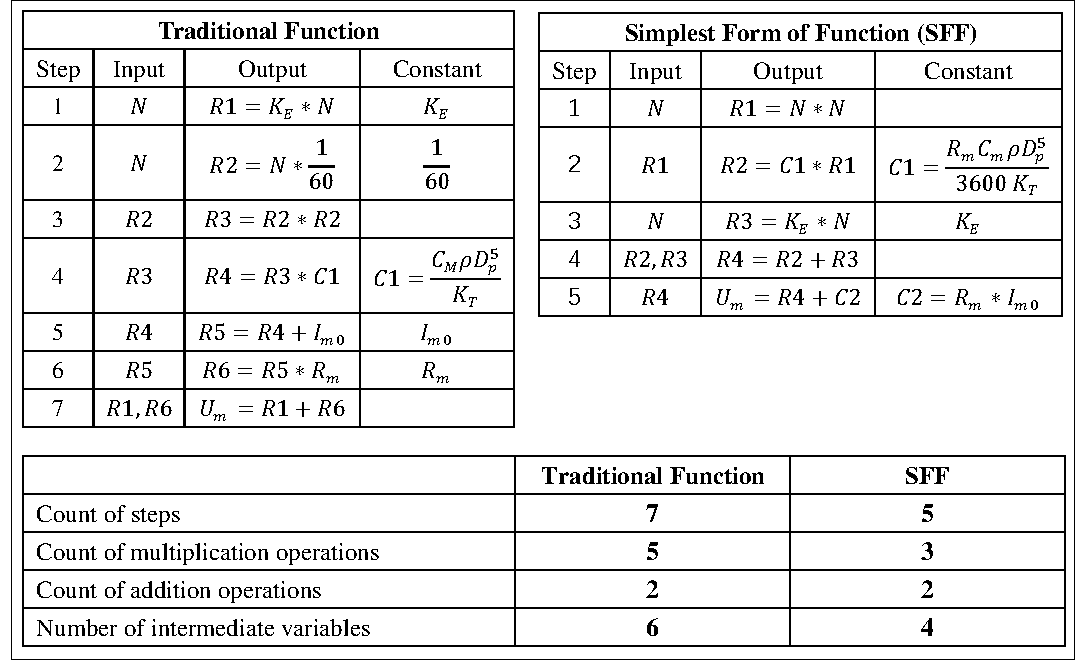
\includegraphics[width=1.0\textwidth]{fig3_CompareTwoMethods.pdf}}
\caption{Comparison of traditional functions and SFF}
\label{fig:fig3_CompareTwoMethods}
\end{figure}
As can be seen from Fig \ref{fig:fig3_CompareTwoMethods}, the new SFF are calculated less and the number of intermediate variables are reduced too.
At the same time, the type of the new SFF is more clearly than old form, it is an unary quadratic function form.

This comparison shows that SFF is a better approach and may greatly improve the efficiency of engineering computing.

We have done equivalent transformations to many original functions, and given the SFF table, see Fig \ref{fig:fig2_SimplestFormFunctions}.
\begin{figure}[H]%[htbp]
\centerline{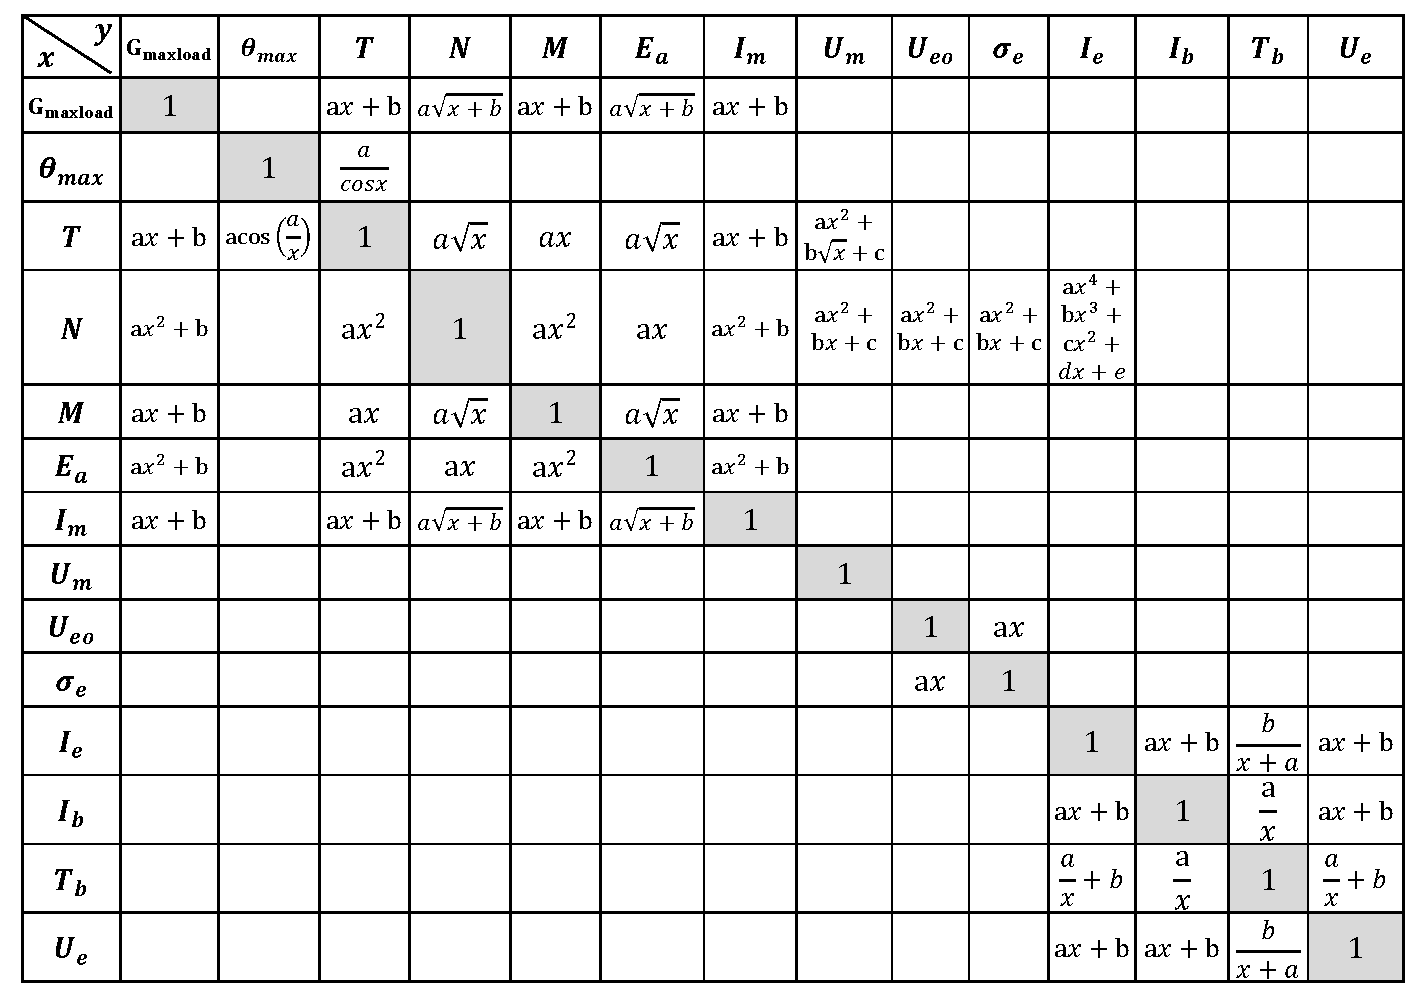
\includegraphics[width=1.0\textwidth]{fig2_SimplestFormFunctions.pdf}}
\caption{Simplest Form of Function Table of Propulsion Subsystem}
\label{fig:fig2_SimplestFormFunctions}
\end{figure}
The first column of the table is the input, and the first row is the output, the a, b, c in the table represent a constant expression in SFF, and the a, b, c in different functions is not the same value, just means they are constant expressions.
We haven’t filled all blank grids because some functions only have mathematical meaning, haven't engineering meaning, and the form is more complicated, so it is not the first priority to complete.
Because we know from VRG that there are calculation paths between any nodes, there should be a function for each grid, and there must be an SFF.
It should be pointed out that any pair of functions that are symmetrical on the main diagonal are mutually inverse.

There are now 14 important variables in total. 
After a rough estimate, the number of formulas that can be obtained is $13 + 12 + ... + 1 = 91$, but in fact some of them are meaningless and there is no need to list them.

\subsection{Formal verification}\label{main:basic:formal}

\subsubsection{Customized automatic tactic}

In the field of engineering control, the most common is the lengthy mathematical formula of the real number type. 
The real number type in the Coq system is constructed with axioms, and the related proofs require a lot of lemmas to rewrite and simplify.
This is a manual proof example of correctness of a function which composited by two functions about thrust $T$ and propeller speed $N$.
\begin{verbatim}
Lemma verify_trans_N_and_T N : 0 < N -> get_N_by_T (get_T_by_N N) = N.
Proof.
  intros H1. unfold get_N_by_T, get_T_by_N.
  remember (rho * C_T * D_p ^ 4) as a.
  unfold Rdiv. rewrite Rinv_r_simpl_m.
  - rewrite sqrt_pow2.
    + rewrite -> Rmult_assoc. rewrite Rinv_r_simpl_m; trivial.
    + apply Rle_mult_inv_pos. trivial. lra.
  - rewrite Heqa.
    apply Rmult_integral_contrapositive. split.
    + apply Rmult_integral_contrapositive. split.
      * apply Rgt_not_eq. apply Rlt_gt; apply gt0_rho.
      * apply Rgt_not_eq. apply Rlt_gt; apply gt0_C_T.
    + apply pow_nonzero; apply Rgt_not_eq; 
      apply Rlt_gt;apply gt0_D_p.
Qed.
\end{verbatim}

It can be seen that this script is cumbersome and poor readable.
We found that many proofs are same pattern, first expand the definition, then use some lemmas to apply, try to use the Ring or Field strategy to auto prove the equality, and try to use the Fourier strategy to auto prove the general inequality.

We packaged these automatic proof technologies and provide a real number proof module named R\_prove.
This module consists of three parts: a table of commonly used lemmas, see Table \ref{tab:reals_lemmas}; custom lemmas; custom strategies.

%\caption{Common lemmas about real Number}
\begin{center}
\begin{tabular}{|l|l|}
\hline
\textbf{Lemma name} & \textbf{Lemma type} \\
\hline
Rlt\_0\_1					& $0 < 1													$ \\
Rmult\_le\_pos              & $0 \le r1 \rightarrow 0 \le r2 \rightarrow 0 \le r1      	$ \\ 
Rmult\_lt\_0\_compat        & $0 < r1 \rightarrow 0 < r2 \rightarrow 0 < r1 * r2   		$ \\ 
Rgt\_not\_eq                & $r1 > r2 \rightarrow r1 \ne r2                			$ \\
Rlt\_le                     & $r1 < r2 \rightarrow r1 \le r2                			$ \\ 
pow\_lt                    	& $0 < x \rightarrow 0 < x ^ n                 				$ \\ 
pow\_nonzero               	& $x \ne 0 \rightarrow x ^ n \ne 0               			$ \\
Rsqr\_sqrt                 	& $0 \le x \rightarrow (sqrt x)^2 = x            			$ \\ 
sqrt\_pow2                 	& $0 \le x \rightarrow sqrt (x ^ 2) = x         			$ \\ 
\hline
\end{tabular}
\label{tab:reals_lemmas}
\end{center}

We use the proof strategy library management command Hint to add strategies to a specified strategy library. 
For example, ``Hint Resolve Rlt\_le : flyctrl.'' adds the strategy ``apply Rlt\_le'' to the flyctrl strategy library. 
Then you can enter ``auto with flyctrl'' to use this automatic proof strategy library.

Among the custom strategies, one of the most commonly used strategies is ``simple\_equation'', which can solve most of the proof problems in PS.
\begin{verbatim}
Ltac simple_equation := intros;
  repeat autounfold with flyctrl; auto with flyctrl; unfold Rdiv;
  autorewrite with flyctrl;try field;try fourier; auto with flyctrl;
  try apply Rmult_le_pos; auto with flyctrl;
  try apply Rmult_integral_contrapositive; auto with flyctrl;
  repeat try split; auto with flyctrl.
\end{verbatim}

The example of manual proof just demonstrated can be done in one step with this strategy.
\begin{verbatim}
Lemma verify_trans_N_and_T' N : 
  0 < N -> get_N_by_T (get_T_by_N N) = N.
  Proof. simple_equation. Qed.
\end{verbatim}

\subsubsection{Verification of equality of function transformation}
It is mainly to verify the definitions of basic inverse functions and derivative functions.

The first is the transformation of the paired basic function and the inverse function, named \verb|verify_trans_XX_and_YY|, where XX and YY represent two variables respectively.

{\small
\begin{verbatim}
Lemma verify_trans_N_and_T N : get_N_by_T (get_T_by_N N) = N.
Lemma verify_trans_N_and_M N : get_N_by_M (get_M_by_N N) = N.
Lemma verify_trans_N_and_E_a N : get_N_by_E_a (get_E_a_by_N N) = N.
Lemma verify_trans_I_m_and_M I_m : get_I_m_by_M (get_M_by_I_m I_m) = I_m.
Lemma verify_trans_sigma_e_and_U_eo sigma_e: 
    get_sigma_e_by_U_eo (get_U_eo_by_sigma_e sigma_e) = sigma_e.
Lemma verify_trans_I_e_and_I_b I_e : get_I_e_by_I_b (get_I_b_by_I_e I_e) = I_e.
Lemma verify_trans_I_b_and_T_b I_b : get_I_b_by_T_b (get_T_b_by_I_b I_b) = I_b.
Lemma verify_trans_I_b_and_U_e I_b : get_I_b_by_U_e (get_U_e_by_I_b I_b) = I_b.
Lemma verify_trans_T_and_G_maxload T : 
    get_T_by_G_maxload (get_G_maxload_by_T T) = T.
Lemma verify_trans_T_and_sigma_max T : 
    get_T_by_theta_max (get_theta_max_by_T T) = T.
\end{verbatim}
}

Then let's verify the definition of the derived function, and named it \verb|verify_XXX|, where XXX represents the name of the derived function.

{\small
\begin{verbatim}
Lemma verify_get_T_by_M M : get_T_by_M M = get_T_by_N (get_N_by_M M).
Lemma verify_get_M_by_T M : get_M_by_T (get_T_by_M M) = M.
Lemma verify_get_I_m_by_T T : get_I_m_by_T T = get_I_m_by_M (get_M_by_T T).
Lemma verify_get_E_a_by_T T : get_E_a_by_T T = get_E_a_by_N (get_N_by_T T).
Lemma verify_get_U_m_by_T T : get_U_m_by_T T = 
    get_U_m_by_E_a_and_I_m (get_E_a_by_T T) (get_I_m_by_T T).
    
Lemma verify_get_U_m_by_N_and_M N M : get_U_m_by_N_and_M N M =
    get_U_m_by_E_a_and_I_m (get_E_a_by_N N) (get_I_m_by_M M).
Lemma verify_get_U_m_by_N N : get_U_m_by_N N =
    get_U_m_by_N_and_M N (get_M_by_N N).
Lemma verify_get_U_m_by_M M : get_U_m_by_M M =
    get_U_m_by_N_and_M (get_N_by_M M) M.
		
Lemma verify_get_U_eo_by_E_a_and_I_m E_a I_m : 
    get_U_eo_by_E_a_and_I_m E_a I_m = 
    get_U_eo_by_U_m_and_I_m (get_U_m_by_E_a_and_I_m E_a I_m) I_m.
Lemma verify_get_U_eo_by_N N : get_U_eo_by_N N =
    get_U_eo_by_E_a_and_I_m (get_E_a_by_N N) 
    (get_I_m_by_M (get_M_by_N N)).
    
Lemma verify_get_sigma_e_by_E_a_and_I_m E_a I_m : 
    get_sigma_e_by_E_a_and_I_m E_a I_m = 
    get_sigma_e_by_U_eo (get_U_eo_by_E_a_and_I_m E_a I_m).
Lemma verify_get_I_e_by_E_a_and_I_m E_a I_m : get_I_e_by_E_a_and_I_m E_a I_m = 
    get_I_e_by_sigma_e_and_I_m (get_sigma_e_by_E_a_and_I_m E_a I_m) I_m.
Lemma verify_get_I_e_by_T T : get_I_e_by_T T =
    get_I_e_by_E_a_and_I_m (get_E_a_by_T T) (get_I_m_by_T T).
Lemma verify_get_U_e_by_I_e I_e : get_U_e_by_I_e I_e = 
    get_U_e_by_I_b (get_I_b_by_I_e I_e).
Lemma verify_get_T_b_by_I_e I_e : get_T_b_by_I_e I_e = 
    get_T_b_by_I_b (get_I_b_by_I_e I_e).
Lemma verify_get_N_by_U_m U_m : get_U_m_by_N (get_N_by_U_m U_m) = U_m.
Lemma verify_get_N_by_U_eo U_eo : get_U_eo_by_N (get_N_by_U_eo U_eo) = U_eo.

\end{verbatim}
}


\newpage
% ++++++++++++++++++++++++++++++++++++++++++++++++++++++++++++++++++++++++++++++++++++++++++++++++++

\subsection{Example 1: Estimate the longest hovering time}\label{main:example}

\subsubsection{Analysis of the question}
Question: In the hover mode, according to the known parameters, estimate the time of endurance $T_b$, see \cite{qq} P75.

Principle: In the hovering state, the thrust generated by the PS is exactly equal to the total weight of the aircraft.

\subsubsection{General calculation step}
Calculation steps, see \cite{qq} p81-p82:

\begin{enumerate}
\item Calculate the thrust required by a single propeller, simply divide the total mass by the number of propellers.
\begin{equation*}
T = G / n\_ r\label{q_hover.T}
\end{equation*}

\item Calculate the propeller speed
\begin{equation*}
N = get\_ N\_ by\_ T (T) \label{q_hover.N}
\end{equation*}

\item Calculate the propeller torque
\begin{equation*}
M = get\_ M\_ by\_ T (T) \label{q_hover.M}
\end{equation*}

\item Calculate the back-electromotive force of the motor
\begin{equation*}
E_a = get\_ E\_ a\_ by\_ N (N) \label{q_hover.E_a}
\end{equation*}

\item Calculate the input current of the motor
\begin{equation*}
I_m = get\_ I\_ m\_ by\_ M (M) \label{q_hover.I_m}
\end{equation*}

\item Calculate the input voltage of the motor
\begin{equation*}
U_m = get\_ U\_ m\_ by\_ E\_ a\_ and\_ I\_ m (E_a, I_m) \label{q_hover.U_m}
\end{equation*}

\item Calculate the output voltage of the ESC
\begin{equation*}
U_{eo} = get\_ U\_ eo\_ by\_ U\_ m\_ and\_ I\_ m (U_m, I_m) \label{q_hover.U_eo}
\end{equation*}

\item Calculate the ESC throttle
\begin{equation*}
\sigma_e = get\_ sigma\_ e\_ by\_ U\_ eo\_ and\_ U\_ b (U_{eo}, U_b) \label{q_hover.sigma_e}
\end{equation*}

\item Calculate the input current of the ESC
\begin{equation*}
I_e = get\_ I\_ e\_ by\_ I\_ m\_ and\_ sigma\_ e (I_m, sigma_e) \label{q_hover.I_e}
\end{equation*}

\item Calculate the output current of the battery
\begin{equation*}
I_b = get\_ I\_ b\_ by\_ I\_ e (I_e) \label{q_hover.I_b}
\end{equation*}

\item Calculate the hover time
\begin{equation*}
T_b = get\_ T\_ b\_ by\_ I\_ b (I_b) \label{q_hover.T_b}
\end{equation*}

\end{enumerate}


\subsubsection{Direct calculate formulas}
The formula of direct calculation is given here, which provides another way of calculation.

A direct formula, calculate ${N}$.
\begin{equation}
direct\SL N = 60 \sqrt{\frac {G} {\rho D_p^4 C_T n_r}} \label{q_hover.direct_N}
\end{equation}

A direct formula, calculate ${M}$.
\begin{equation}
direct\SL M = \frac{C_M D_p G}{C_T n_r} \label{q_hover.direct_M}
\end{equation}

A direct formula, calculate ${E_a}$.
\begin{equation}
direct\SL E\SL a = 60 K_{E} \sqrt{\frac {G} {\rho D_p^4 C_T n_r}} \label{q_hover.direct_E_a}
\end{equation}

A direct formula, calculate ${I_m}$.
\begin{equation}
direct\SL I\SL m = \frac{C_M D_p G}{C_T n_r K_T} + {I_{m0}} \label{q_hover.direct_I_m}
\end{equation}

A direct formula, calculate ${U_m}$.
\begin{equation}
direct\SL U\SL m = 60 K_{E}\sqrt{\frac {G} {\rho D_p^4 C_T n_r}} 
	+ R_m \left(\frac{C_M D_p G}{C_T K_T n_r} + {I_{m0}}\right) \label{q_hover.direct_U_m}
\end{equation}

A direct formula, calculate ${U_{eo}}$.
\begin{equation}
direct\SL U\SL eo = 60 K_{E}\sqrt{\frac {G} {\rho D_p^4 C_T n_r}} 
	+ (R_m + R_e) \left(\frac{C_M D_p G}{C_T K_T n_r} + {I_{m0}}\right)
	\label{q_hover.direct_U_eo}
\end{equation}

A direct formula, calculate ${\sigma_{e}}$.
\begin{equation}
direct\SL sigma\SL e = \frac{60 K_{E}\sqrt{\frac {G} {\rho D_p^4 C_T n_r}} 
	+ (R_m + R_e) \left(\frac{C_M D_p G}{C_T K_T n_r} + {I_{m0}}\right)}{U_b}
	\label{q_hover.direct_sigma_e}
\end{equation}

A direct formula, calculate ${I_{e}}$.
\begin{equation}
direct\SL I\SL e = \frac{60 K_{E}\sqrt{\frac {G} {\rho D_p^4 C_T n_r}} 
	+ (R_m + R_e) \left(\frac{C_M D_p G}{C_T K_T n_r}+ {I_{m0}}\right)}{U_b} 
	\left(\frac{C_M D_p G}{C_T n_r K_T} + {I_{m0}}\right)
	\label{q_hover.direct_I_e}
\end{equation}

A direct formula, calculate ${I_{b}}$.
\begin{equation}
direct\SL I\SL b = n_r \left(\frac{60 K_{E}\sqrt{\frac {G} {\rho D_p^4 C_T n_r}} 
	+ (R_m + R_e) \left(\frac{C_M D_p G}{C_T K_T n_r} + {I_{m0}}\right)}{U_b} 
	\left(\frac{C_M D_p G}{C_T n_r K_T} + {I_{m0}}\right)
	\right)
	+ I_{other}
	\label{q_hover.direct_I_b}
\end{equation}

A direct formula, calculate ${U_{e}}$.
\begin{equation}
direct\SL U\SL e = U_b - \left(n_r \left(\frac{60 K_{E}\sqrt{\frac {G} {\rho D_p^4 C_T n_r}} 
	+ (R_m + R_e) \left(\frac{C_M D_p G}{C_T K_T n_r} + {I_{m0}}\right)}{U_b} 
	\left(\frac{C_M D_p G}{C_T n_r K_T} + {I_{m0}}\right)  
	\right)
	+ I_{other}\right) R_b
	\label{q_hover.direct_U_e}
\end{equation}

A direct formula, calculate ${T_b}$.
\begin{equation}
direct\SL T\SL b = \frac{C_b - C_{min}}
	{n_r \left(\frac{60 K_{E}\sqrt{\frac {G} {\rho D_p^4 C_T n_r}} 
	+ (R_m + R_e) \left(\frac{C_M D_p G}{C_T K_T n_r} + {I_{m0}}\right)}{U_b} 
	\left(\frac{C_M D_p G}{C_T n_r K_T} + {I_{m0}}\right)
	\right)
	+ I_{other}} 
	\frac{60}{1000} \label{q_hover.direct_T_b}
\end{equation}

Note that these formulas are not so handsome but really correct.
If we transform them using the SFF method, then we will get a more elegant form.

\subsubsection{Vefiry direct formulas}

Verify that the results calculated by general method are equal to the new given direct fomulas, 
so we can ensure that the new formulas are reliable.

\begin{verbatim}
Lemma direct_N_correct : direct_N = N.
Lemma direct_M_correct : direct_M = M.
Lemma direct_E_a_correct : direct_E_a = E_a.
Lemma direct_I_m_correct : direct_I_m = I_m.
Lemma direct_U_m_correct : direct_U_m = U_m.
Lemma direct_U_eo_correct : direct_U_eo = U_eo.
Lemma direct_sigma_e_correct : direct_sigma_e = sigma_e.
Lemma direct_I_e_correct : direct_I_e = I_e.
Lemma direct_I_b_correct : direct_I_b = I_b.
Lemma direct_U_e_correct : direct_U_e = U_e.
Lemma direct_T_b_correct : direct_T_b = T_b.
\end{verbatim}

\newpage
% ++++++++++++++++++++++++++++++++++++++++++++++++++++++++++++++++++++++++++++++++++++++++++++++++++

\subsection{Example 2: Estimate system effencicy at max throttle}

\subsubsection{Analysis of the question}
Question: Solve the motor voltage, motor current, propeller speed and system efficiency under the maximum throttle mode.

Principle: Under the maximum throttle, the electric throttle is equal to 1. 
At this time, multiple equations are combined to solve the result.

For the solution of the key variable "propeller speed N", literature \cite{qq}[p71, 4.30] gives a system of equations,
A numerical iteration method is proposed to solve the problem, but the final expression is not given.
The author gives the formula of direct calculation.


\subsubsection{General calculation step}

\begin{enumerate}

\item Given the throttle, see \cite{qq}[p.71, 4.30]
\begin{equation}
sigma_e = 1 \label{q_maxthrottle.sigma_e}
\end{equation}

\item Calculate $U_{eo}$
\begin{equation}
U_{eo} = get\SL U\SL eo\SL by\SL sigma\SL e (sigma_e) \label{q_maxthrottle.U_eo}
\end{equation}

\item Calculate $N$
\begin{equation}
N = get\SL N\SL by\SL U_{eo} (U_{eo}) \label{q_maxthrottle.N}
\end{equation}

\item Calculate $M$
\begin{equation}
M = get\SL M\SL by\SL N (N) \label{q_maxthrottle.M}
\end{equation}

\item Calculate $I_m$
\begin{equation}
I_m = get\SL I\SL m\SL by\SL M (M) \label{q_maxthrottle.I_m}
\end{equation}

\item Calculate $I_e$
\begin{equation}
I_e = get\SL I\SL e\SL by\SL I\SL m\SL and\SL sigma\SL e (I_m, sigma_e) \label{q_maxthrottle.I_e}
\end{equation}

\item Calculate $I_e$
\begin{equation}
I_b = get\SL I\SL b\SL by\SL I\SL e (I_e) \label{q_maxthrottle.I_b}
\end{equation}

\item Calculate $\eta$
\begin{equation}
\eta = get\SL eta\SL by\SL M\SL and\SL N\SL and\SL I\SL b (M, N, I_b) \label{q_maxthrottle.eta}
\end{equation}

\end{enumerate}


\newpage
% ++++++++++++++++++++++++++++++++++++++++++++++++++++++++++++++++++++++++++++++++++++++++++++++++++

\subsection{Example 3: Estimate maximum load and maximum pitch Angle}

\subsubsection{Analysis of the question}
Question: Calculate the maximum load weight and the maximum pitch Angle of multiple rotors with a certain safety margin (e.g., 20\%) reserved for throttle commands.

Principle: Use the maximum throttle in safe mode, here 0.8, then combine multiple equations to solve the result.

For the solution of the key variable "propeller speed N", literature \cite{qq}[p73, 4.33] gives a system of equations,
A numerical iteration method is proposed to solve the problem, but the final expression is not given.
This problem is similar to the "maximum throttle mode" problem, and the direct calculation formula is given.

\subsubsection{General calculation step}

\begin{enumerate}

\item Given the throttle, see \cite{qq}[p.73, 4.33]
\begin{equation}
sigma_e = 0.8 \label{q_maxload.sigma_e}
\end{equation}

\item Calculate $U_{eo}$
\begin{equation}
U_{eo} = get\SL U\SL eo\SL by\SL sigma\SL e (sigma_e) \label{q_maxload.U_eo}
\end{equation}

\item Calculate $N$
\begin{equation}
N = get\SL N\SL by\SL U_{eo} (U_{eo}) \label{q_maxload.N}
\end{equation}

\item Calculate $T$
\begin{equation}
T = get\SL T\SL by\SL N (N) \label{q_maxload.T}
\end{equation}

\item Calculate $G_{maxload}$
\begin{equation}
G_{maxload} = get\SL G\SL maxload\SL by\SL T (T) \label{q_maxload.G_maxload}
\end{equation}

\item Calculate $\theta_{max}$
\begin{equation}
\theta_{max} = get\SL \theta\SL max\SL by\SL T (T) \label{q_maxload.theta_max}
\end{equation}

\end{enumerate}

\newpage
% ++++++++++++++++++++++++++++++++++++++++++++++++++++++++++++++++++++++++++++++++++++++++++++++++++

\subsection{Example 4: Estimate maximum flat flight speed and distance}

\subsubsection{Analysis of the question}

Question: Designers are concerned about two performance metrics: maximum flat flight speed and distance.
The function relationship between pitch Angle and flight speed can be obtained after the model is established by force analysis.
The solving method given by the author of the original book is numerical iteration method, but the author wants to try to find a better formula for direct calculation.
The knowledge of derivative and extreme point is introduced to try to solve the extreme point.
There is no conclusion and the issue is on hold.

Principle: The function relationship between flight speed and pitch Angle is established firstly, and then the pitch Angle when the maximum flight speed is obtained is solved. Then other parameters are easy to be solved.
Similarly, the maximum flight distance can also be established as a function of pitch Angle, which can be solved in the same way.


\newpage
% ++++++++++++++++++++++++++++++++++++++++++++++++++++++++++++++++++++++++++++++++++++++++++++++++++


\section{Summary}

In order ot realize control system as computer software, it is necessary to extract the exisiting engineering knowledge into the reference manual of software programming model required by computer programming.
This process is traditionally completed by people manully, and its reliability cannot be guaranteed.
We use the theorem prover COQ to gradually establish a reliable knowledge base for the control system from the bottom level in the way of mathematical reasoning.
At the same time, we also get a reliable model that has been formally verified.
We take the flight control system of small unmanned aerial vehicle as the research object, and analyze the control principle and algorithm of each subsystem.
The research object of this chapter is propulsion system modeling.

In future work, we will use program generation technology to automatically generate high reliability control system software from this model.

\begin{thebibliography}{99}
\bibitem{qq} Quan, Q. . Introduction to Multicopter Design and Control. Springer Singapore, 2017.
%\bibitem{air} 徐敏. 空气动力学基础(第2版). 西北工业大学出版社
%\bibitem{fly} 高压奎. 飞行仿真技术. 上海交通大学出版社
%\bibitem{perf} 田勇. 飞机性能工程学. 科学出版社
\bibitem{practical} Shi, D. , et al. "A Practical Performance Evaluation Method for Electric Multicopters." IEEE/ASME Transactions on Mechatronics 22.3(2017):1337-1348.
\end{thebibliography}

\end{document}
